\documentclass{beamer}
\usetheme{Hannover}
\setbeamercovered{transparent}
\renewcommand{\Roman}[1]{$\overline{\textsf{\small{\MakeUppercase{\romannumeral #1}}}}$}
\setbeamertemplate{navigation symbols}{}


% Chicago Bibliography Formatting
\usepackage[
  autocite = footnote,
  sorting=ynt,
  annotation]
  {biblatex-chicago}
   
\renewcommand{\bibfont}{\normalsize}
\addbibresource{Bibliography.bib}

% Language and Text Formatting
\usepackage[utf8]{inputenc}
\usepackage[T1]{fontenc}
\usepackage{microtype}
\usepackage[greek, english]{babel}
  \babeltags{en = english}
  \babeltags{el = greek}
\usepackage{csquotes} %idk, babel asks for it ¯\_(ツ)_/¯
\usepackage{teubner}


% Figure Formatting
\usepackage{multicol}
\usepackage{booktabs}
\usepackage{graphicx}
\usepackage{tikz}

% Title Page
\title{This Great Flood of Words\thanks{Rep. 1: 344 d1}}
\author{Thomas Broadwater}
\date{\today}

%%%%%%%%%%%%%%%%%%%%%%%%%%%%%%%%%%%%%%%%%%%%%%%%%%%%%%%%%%%%%%%%%%%%%%%%%%%%%%%%

\usepackage{Sweave}
\begin{document}
\Sconcordance{concordance:GreatSlideshow.tex:GreatSlideshow.Rnw:%
1 41 1 1 0 6 1 1 11 1 19 1 12 108 1 1 69 20 1 1 2 12 0 1 2 35 1 2 2 5 1 %
1 84 16 1 2 2 5 1 2 2 5 1 1 19 4 1 1 3 4 0 1 2 23 1 1 8 1 2 5 1 1 9 1 2 %
1 1 1 94 22 1 1 2 12 0 1 2 18 1 2 2 9 1 2 2 18 1 1 23 2 2 5 1 1 22 2 2 %
17 1 1 8 1 2 2 1}


\begin{frame}
\titlepage
\end{frame}




\section{Introduction} % ----------------------------------------------------- %

\subsection{Phasal Analysis} % - - - - - - - - - - - - - - - - - - - - - - - - %

\begin{frame}
\frametitle{Phasal Analysis \Roman{1}}
\begin{itemize}
\item Register: style based on context
\item Phase: like a subregister
  \begin{itemize}
  \item unit of discourse
  \item consistent style based on specifics
    \begin{itemize}
    \item familiarity, topic, venue, etc.
  \end{itemize}
  \end{itemize}
\end{itemize}
\end{frame}



\begin{frame}
\frametitle{Phasal Analysis \Roman{2}}
\begin{itemize}
\item Phases: characterized by shared features
  \begin{itemize}
  \item word choice, mood (indicative, imperative, etc.)
  \item topic, sentence length
  \end{itemize}
\end{itemize}
\end{frame}



\begin{frame}
\frametitle{Goals}
\begin{enumerate}
\item broad phasal analysis of Rep.1
\item demonstration of programmatic methods
\end{enumerate}
\vspace*{\fill}
\hspace*{\fill}
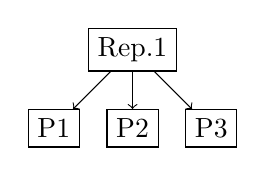
\begin{tikzpicture}
\centering
\node[draw, anchor = south] (Rep1) at (0,0) {Rep.1};
  \node[draw, anchor = north, below of = Rep1] (P2) {P2};
    \node[draw, anchor = north, left of = P2] (P1) {P1};
    \node[draw, anchor = north, right of = P2] (P3) {P3};
\draw[->] (Rep1) -- (P2);
\draw[->] (Rep1) -- (P1);
\draw[->] (Rep1) -- (P3);
\end{tikzpicture}
\hspace*{\fill}
\vspace*{\fill}
\end{frame}



\subsection{R Scripting} % - - - - - - - - - - - - - - - - - - - - - - - - - - %

\begin{frame}
\frametitle{Code \Roman{1}}
\begin{itemize}
\item R script written for analysis
\item analyzes on turn-by-turn basis
\item searches for 3 key metrics
  \begin{itemize}
  \item turn density (sentences per turn)
  \item turn length (words per turn)
  \item turn sentiment (sentimental impact per turn)
  \end{itemize}
\end{itemize}
\end{frame}



\begin{frame}
\frametitle{Code \Roman{2}}
\begin{itemize}
\item requirements for this script:
  \begin{itemize}
  \item ``stop words''
  \item ``lemmatizer''
  \item ``sentiment dictionary''
  \end{itemize}
\end{itemize}
\end{frame}



\begin{frame}
\frametitle{Caveat Emptor\dots}
\begin{itemize}
\item Do these resources exist for Ancient Greek?
  \begin{itemize}
    \item \textit{No}
    \item And they typically require whole departments to build
    \item Using translation by GMA Grube and CDC Reeve (1992)
  \end{itemize}
\end{itemize}
\end{frame}



\section{The Study} % -------------------------------------------------------- %

\subsection{Turn Density}  % - - - - - - - - - - - - - - - - - - - - - - - - - %


\begin{frame}
\frametitle{Turn Density \Roman{1}}
\begin{itemize}
\item Turn Density: number of sentences per turn
  \begin{itemize}
  \item i.e. consecutive sentences per speaker
  \end{itemize}
\item need a broad picture
  \begin{itemize}
  \item mean, median, mode, standard deviation
  \item global (i.e. across Rep.1)
  \item per speaker
  \end{itemize}
\end{itemize}
\end{frame}



\begin{frame}[fragile]
\frametitle{Turn Density \Roman{2}}
\begin{Schunk}
\begin{Soutput}
# A tibble: 6 × 5
  speaker      mean median  mode    sd
  <chr>       <dbl>  <dbl> <int> <dbl>
1 global       1.69    1       1 1.79 
2 cleitophon   1.33    1       1 0.577
3 glaucon      1.25    1       1 0.463
4 polemarchus  1.75    1.5     1 0.957
5 socrates     1.99    1       1 1.90 
6 thrasymacus  1.41    1       1 1.72 
\end{Soutput}
\end{Schunk}
\end{frame}



\begin{frame}
\frametitle{Turn Density \Roman{3}}
\begin{itemize}
\item What does any of that mean?
  \begin{itemize}
  \item Very little until you run it through a t-test
  \item I won't make you suffer that
  \end{itemize}
\end{itemize}
\end{frame}



\begin{frame}
\frametitle{Turn Density \Roman{4}}
\begin{itemize}
\item means, medians, and modes are too regular
  \begin{itemize}
  \item makes sense: call-and-response style
  \end{itemize}
\item statistically significant standard deviations:
  \begin{itemize}
  \item Socrates and Thrasymachus
  \item also widest range of turn densities
  \end{itemize}
\end{itemize}
\end{frame}



\begin{frame}
\frametitle{Turn Density \Roman{5}}
\includegraphics{GreatSlideshow-006}
\end{frame}



\subsection{Turn Length} % - - - - - - - - - - - - - - - - - - - - - - - - - - %


\begin{frame}
\frametitle{Turn Length \Roman{1}}
\begin{itemize}
\item Turn Length: number of words per turn
\item different calculations, same results
  \begin{itemize}
  \item means, medians, modes all too regular
  \item Socrates and Thrasymachus show statistically significant standard deviations
  \end{itemize}
\end{itemize}
\end{frame}



\begin{frame}
\frametitle{Turn Length \Roman{2}}
\includegraphics{GreatSlideshow-008}
\end{frame}



\begin{frame}[fragile]
\frametitle{Turn Size Index \Roman{1}}
\includegraphics{GreatSlideshow-Turn_Length}
\end{frame}



\subsection{Size Index}  % - - - - - - - - - - - - - - - - - - - - - - - - - - %



\begin{frame}[fragile]
\frametitle{Index \Roman{1}}
\begin{block}{Density / Length Correlation Coefficient}
\begin{Schunk}
\begin{Soutput}
[1] 0.9294758
\end{Soutput}
\end{Schunk}
\end{block}
\end{frame}



\begin{frame}
\frametitle{Index \Roman{2}}
\begin{itemize}
\item density and length are closely correlated
\item new variable: Size index
  \begin{itemize}
  \item per-turn average of density and length
  \end{itemize}
\end{itemize}
\end{frame}


%%% THOMAS THESE ARE THE TABLES YOU NEED FOR SIZE INDEXING LATER
%%% FIRST ONE IS A COMPOSIT GEOM_SMOOTH
%%% TOP IS LENGTH, BOTTOM IS DENSITY, MIDDLE DASHED IS SIZE
%%% SECOND ONE IS THE SIZE HISTOGRAM W/ MOVING AVERAGE

\begin{frame}[fragile]
\frametitle{Index \Roman{3}}
\includegraphics{GreatSlideshow-012}
\end{frame}



\begin{frame}[fragile]
\frametitle{Index \Roman{4}}
\includegraphics{GreatSlideshow-013}
\end{frame}




\subsection{Sentiment Analysis}  % - - - - - - - - - - - - - - - - - - - - - - %

\begin{frame}
\frametitle{Sentiment Analysis \Roman{1}}
\begin{itemize}
\item Sentiment Analysis: measuring vibes
\item AFINN Lexicon
  \begin{itemize}
  \item Ranks sentiment from -5 to +5
  \item $-5$: most negative
  \item $+5$: most positive
  \item $0$: neutral
  \end{itemize}
\end{itemize}
\end{frame}



\begin{frame}[fragile]
\frametitle{Sentiment Analysis \Roman{2}}
\begin{Schunk}
\begin{Soutput}
# A tibble: 6 × 5
  speaker       mean median  mode    sd
  <chr>        <dbl>  <dbl> <dbl> <dbl>
1 global       0.415  1         1  1.43
2 cleitophon   2      2         2 NA   
3 glaucon     -0.5   -0.5      NA  2.12
4 polemarchus  0.519  1        NA  1.34
5 socrates     0.433  0.775     2  1.50
6 thrasymacus  0.380  1         1  1.30
\end{Soutput}
\end{Schunk}
\end{frame}



\begin{frame}
\frametitle{Sentiment Analysis \Roman{3}}
\begin{itemize}
\item more interesting results:
  \begin{itemize}
    \item Socrates and Thrasymachus show statistically significant means
    \item Polemarchus, Socrates, and Thrasymachus show statistically significant standard deviations
  \end{itemize}
\end{itemize}
\end{frame}



\begin{frame}[fragile]
\frametitle{Sentiment Analysis \Roman{4}}
\includegraphics{GreatSlideshow-016}
\end{frame}



\section{The Results} % ------------------------------------------------------ %

\subsection{Bars}  % - - - - - - - - - - - - - - - - - - - - - - - - - - - - - %

\begin{frame}[fragile]
\frametitle{Results \Roman{1}}
\includegraphics{GreatSlideshow-017}
\end{frame}


\begin{frame}
\frametitle{Results \Roman{2}}
\begin{itemize}
\item size index shows turning point between x100 and x150
  \begin{itemize}
  \item corresponding points on sentiment chart: x54 and x94
  \item corresponding with 347.d7 T40 and 348.e5 S73
  \end{itemize}
\item sentiment analysis shows slight inverse turning point in same range
\end{itemize}
\end{frame}



\begin{frame}[fragile]
\frametitle{Results \Roman{3}}

\includegraphics{GreatSlideshow-019}
\end{frame}



\begin{frame}[fragile]
\frametitle{Results \Roman{4}}

\includegraphics{GreatSlideshow-021}
\end{frame}



\begin{frame}
\frametitle{Results \Roman{5}}
\begin{itemize}
\item 347.e6 G4 to 348.b6 G8
\item Following Thrasymachus' ``great flood of words'' speech
\end{itemize}

\begin{block}{343.a2 T42}
Tell me, Socrates, do you still have a wet nurse?
\end{block}
\end{frame}

\begin{frame}[fragile]
\frametitle{Results \Roman{6}}
\includegraphics{GreatSlideshow-022}
\end{frame}

\end{document}
